\subsubsection{\syscall{WriteProcessMemory} external modifications}
\gls{WPM} is a function available through the \emph{Windows} \gls{API}. This function allows to write into the virtual memory of a target process and allows modification of existing data or code. There are several ways to make use of this function. \gls{WPM} is used for \gls{DLL} injection with the \syscall{CreateRemoteThread} function, code modification and function detouring. This method can be found in Figure~\ref{fig:attacks_external} in node [1.1].
\paragraph{\syscall{CreateRemoteThread} \gls{DLL} Injection}
\glspl{DLL} can be loaded into a target process by loading their path into the target memory with \gls{WPM} and creating a new thread via \syscall{CreateRemoteThread} that calls \syscall{LoadLibrary}. This kind of attack can be used on any process running under the same integrity level and therefore is widely used in game cheating.

\paragraph{Step 1} 
At first, a handle to the target process is requested via \syscall{OpenProcess} with \syscall{PROCESS\_VM\_WRITE} and \syscall{PROCESS\_VM\_OPERATION} access rights. These access rights are required to execute the \gls{WPM} function. If the permissions are missing, \gls{WPM} is not able to modify the virtual memory of the target process. Virtual memory protection flags do not have to be changed manually, as this is already happening inside \gls{WPM}. 

\paragraph{Step 2} 
A large enough amount of memory is allocated inside the target process with \syscall{VirtualAllocEx}, to hold the full path of the \gls{DLL}. 

\paragraph{Step 3}
Next, \gls{WPM} is used to transfer the \gls{DLL} path into the target memory space.

\paragraph{Step 4}
The injection can be completed by calling \syscall{CreateRemoteThread}, which loads the \gls{DLL} with the \syscall{LoadLibrary} function. The allocated memory segment is used as a parameter for the \syscall{LoadLibrary} function call. 

\paragraph{Step 5}
With the loaded \gls{DLL}, arbitrary code can get executed by the \gls{DLL} inside the attacked process, either via using \syscall{CreateRemoteThread} again or via the \gls{DLL}'s entry point.


An example of a basic \gls{DLL} injection using \gls{WPM} and \syscall{CreateRemoteThread} can be found in Appendix~\ref{appendix:writeprocessmemory}. \emph{Chrome} shows no existing defense mechanisms against direct memory modification.
\paragraph{Code modification with \syscall{WriteProcessMemory}}
A second way to make use of \syscall{WriteProcessMemory} is modifying the targets code inside memory, to execute different instructions than intended. This technique is also commonly known as function hooking or function detouring \cite{codeproject_hooking}, which is described in the next paragraph. 
\paragraph{Function detouring}
\begin{figure}[!htbp]
	\centering
	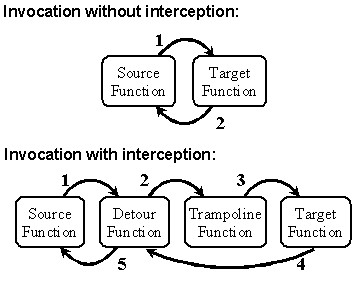
\includegraphics[scale=0.7]{sections/background/attacks/fig_detours.png}
	\caption{This figure shows the change in control flow of a detoured function \cite{detours}}
	\label{fig:detours}
\end{figure}


Function detouring has been greatly simplified by the Detours\cite{msdetours} library of Microsoft, but can also be achieved by memory modification with \syscall{WriteProcessMemory} or assembly code. Figure \ref{fig:detours} shows the difference between a function before and after detouring. The function call at the top shows a invocation without interception. The source function calls the target function without any indirection and after the code of the target function has been executed, returns to the calling source function. Detouring makes use of this structure by placing a detour and a trampoline function in between these calls. The source function will now use an indirect call to the target function, by first calling the detour part, which gives space to execute arbitrary code. To do that, a \syscall{jmp} instruction is placed at the beginning of the function, and the original instructions are saved and copied to the trampoline function. After that, the detour function continues with the trampoline function, which executes the copied instructions and ensures that the target function works as if there was no detour placed. Finally, the whole function stack will return, this time skipping the trampoline function, as it was just used to hold the copied instructions.